% =========================================================================
% Appendix G — cross-domain integration (RTSC<->FUSION<->ANTIMATTER<->CERN).
% FILLED. folds UFO/meta/cross-domain-mega.md:
%   the stage->sibling->reuse-atom dependency graph, the NEXUS.tape reuse
%   edges, the triple-SSOT B*=sigma*tau=48 arithmetic-coincidence (OBSERVED
%   not PROVEN), the current_loop_offaxis substrate-of-substrates spine,
%   absorb=manifest-only, and a pgfplots B*=48 recurrence + reuse-edge chart.
% =========================================================================
\section{Cross-Domain Integration --- the RTSC$\leftrightarrow$FUSION$\leftrightarrow$ANTIMATTER$\leftrightarrow$CERN Reuse Lattice}
\label{app:integration}

This appendix folds the full cross-domain reuse lattice that the
4-domain integration map (\S\ref{sec:intmap}) summarizes. It gives the
stage$\to$sibling-domain$\to$reuse-atom dependency graph in full, the
\texttt{NEXUS.tape} reuse-edge catalogue (@D~d19), and the honest
interpretation of the recurring lattice constant
$B^{*}=\sigma\!\cdot\!\tau=48$. The integer $48$ recurs as the RTSC
upper critical field, the FUSION Lawson design target, and the UFO
Meissner-lift design field; it factors as the $n\!=\!6$ divisor product
$\sigma(6)\!\cdot\!\tau(6)=12\!\cdot\!4$. \textbf{This is an
arithmetic-reuse observation, not a proof of integrated physics}:
the integer closes (checkable via \texttt{lattice\_check.hexa}), but its
cross-domain agreement is a NEXUS reuse-edge observation, not a
demonstrated unification. The CERN edge (acceleration/deceleration
ladder feeding the ANTIMATTER positron source) is a \emph{candidate}
edge. UFO absorbs the entire lattice as a \emph{manifest only} --- zero
new physics atoms.

% -------------------------------------------------------------------------
\subsection{The stage $\to$ sibling $\to$ reuse-atom dependency graph}
\label{app:int-graph}

Table~\ref{tab:int-graph} is the dependency graph, transcribed from
\texttt{UFO/meta/cross-domain-mega.md} \S2.1. Each lower rung stands on a
sibling domain's verified atom; CERN is the candidate infrastructure edge.

\begin{table}[h]
\centering
\footnotesize
\setlength{\tabcolsep}{4pt}
\begin{tabular}{@{}l l >{\raggedright\arraybackslash}m{3.6cm} >{\raggedright\arraybackslash}m{3.0cm} c@{}}
\toprule
\textbf{stage} & \textbf{sibling} & \textbf{substrate role} & \textbf{reuse atom} & \textbf{tier} \\
\midrule
\textcircled{\scriptsize 1} hover & RTSC & 48\,T fringe $\to$ Meissner lift & \texttt{ioffe\_loop\_bz}, \texttt{current\_loop\_offaxis} & \tierGreen \\
\textcircled{\scriptsize 2} cruise & FUSION & D--T Lawson + MHD $F{=}J{\times}B{\times}V$ & \texttt{triple\_product} & \tierGreen/\tierYellow \\
\textcircled{\scriptsize 3} orbital & ANTIMATTER & $\bar pp{\to}2\gamma$ $\to$ rel.\ exhaust $c/g$ & \texttt{pair\_threshold\_total}, \texttt{rel\_kinetic\_from\_p} & \tierGreen/\tierYellow \\
(infra) & CERN & accel/decel ladder, rel.\ kinematics ($e^+$) & \texttt{accelerator} (plasma-wakefield) & candidate \\
\bottomrule
\end{tabular}
\caption{The stage$\to$sibling$\to$reuse-atom graph
(\texttt{UFO/meta/cross-domain-mega.md}). Citations resolve to the
\texttt{UFO/verify/stage\{1,2,3\}-*.md} ledgers (\tierGreen\ landed). UFO
contributes no atoms of its own --- it is an integration carrier.}
\label{tab:int-graph}
\end{table}

% -------------------------------------------------------------------------
\subsection{The NEXUS reuse-edge catalogue}
\label{app:int-edges}

The reuse spine is recorded in \texttt{NEXUS.tape}
(Table~\ref{tab:int-edges}). The load-bearing observation is that one
magnetic-field Green's function --- \verb|current_loop_offaxis| (elliptic
$K/E$ on-axis $B$) --- is the \emph{substrate-of-substrates}: it flows
from NOVEL-TOOL into RTSC and ANTIMATTER, and RTSC's $\zeta\!=\!0$
specialization \verb|ioffe_loop_bz| flows into UFO Stage-1. Four domains
sharing one field kernel is the actual reuse backbone of the lattice.

\begin{table}[h]
\centering
\footnotesize
\setlength{\tabcolsep}{4pt}
\begin{tabular}{@{}l >{\raggedright\arraybackslash}m{3.4cm} >{\raggedright\arraybackslash}m{3.6cm} c@{}}
\toprule
\textbf{edge} & \textbf{provides $\to$ reused-by} & \textbf{shared primitive} & \textbf{status} \\
\midrule
e1 & NOVEL-TOOL $\to$ RTSC & \texttt{current\_loop\_offaxis} ($K/E$ Green fn) & tier-2 verified \\
e2 & NOVEL-TOOL $\to$ ANTIMATTER & $\to$ Ioffe trap depth 0.35\,K & tier-2 verified \\
e3 & RTSC $\to$ ANTIMATTER & getdp 4.0 solenoid toolchain & tier-2 verified \\
(UFO) & RTSC $\to$ UFO~S1 & \texttt{ioffe\_loop\_bz} ($\zeta{=}0$ special.) & tier-2 verified \\
(UFO) & FUSION $\to$ UFO~S2 & \texttt{triple\_product} (Lawson) & tier-2 verified \\
(UFO) & ANTIMATTER $\to$ UFO~S3 & \texttt{pair\_threshold\_total}, \texttt{rel\_kinetic\_from\_p} & tier-2 verified \\
c1 & CERN $\leftrightarrow$ ANTIMATTER & rel.\ kinematics + decel ladder ($e^+$) & candidate (no code reuse) \\
\bottomrule
\end{tabular}
\caption{The \texttt{NEXUS.tape} reuse-edge catalogue (@D~d19). The CERN
edge c1 is a candidate (no shared code yet); all others are tier-2
verified reuse. \texttt{current\_loop\_offaxis} appears in three edges
(e1, e2, and the UFO~S1 specialization) --- the field kernel that ties
the lattice together.}
\label{tab:int-edges}
\end{table}

% -------------------------------------------------------------------------
\subsection{The triple-SSOT $B^{*}=\sigma\!\cdot\!\tau=48$ coincidence}
\label{app:int-bstar}

\texttt{CROSS-DOMAIN-MEGA.md} \S8.1 records a triple-SSOT constant table:
\begin{equation}
B^{*}=\sigma(6)\!\cdot\!\tau(6)=12\cdot4=48
\;:\;\;
\underbrace{\SI{48}{\tesla}}_{\text{RTSC }H_{c2}\text{ (Pauli)}}
=\underbrace{\SI{48}{\tesla}}_{\text{FUSION Lawson target}}
=\underbrace{\SI{48}{\tesla}}_{\text{UFO Meissner lift}} .
\label{eq:int-bstar}
\end{equation}
The integer $48$ closes exactly (it is a verifiable divisor product,
checkable via \verb|UFO/verify/lattice_check.hexa|), and the recurrence
across the three domains is visualized in Fig.~\ref{fig:int-bstar}.
\textbf{We flag it explicitly as an arithmetic-reuse observation, not a
proof of integrated physics.} The agreement is a NEXUS reuse-edge
observation; it does not show the three fields are the \emph{same} field
or that the integration is physically real. This is the same separation
the capstone keeps for the Stage-4--7 lattice integers: bookkeeping
closure $\ne$ empirical truth. The larger ``$\Omega_{\text{mega}}=480$''
mega-integration figure from the source is, identically, an
arithmetic-reuse observation and is \emph{not} an integrated-physics
claim.

\begin{figure}[h]
\centering
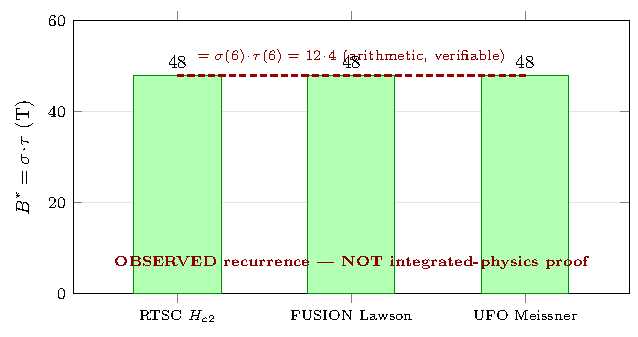
\includegraphics[width=0.84\linewidth]{figures/fig09_bstar_recurrence.pdf}
\caption{The $B^{*}=\sigma\!\cdot\!\tau=48$ recurrence across three
domains (Eq.~\eqref{eq:int-bstar}): RTSC $H_{c2}$, the FUSION Lawson
design target, and the UFO Meissner-lift design field all sit at the same
integer $48$, which factors as $\sigma(6)\!\cdot\!\tau(6)=12\!\cdot\!4$.
The bars are equal \emph{by arithmetic} (a verifiable divisor product),
shown in green; the red annotation marks the honest caveat ---
\textbf{the cross-domain agreement is an observation of the bookkeeping,
not a demonstrated unification of the three physics}. The integer
closes; the physics it points to is a separate, open question.}
\label{fig:int-bstar}
\end{figure}

% -------------------------------------------------------------------------
\subsection{Honest scope --- absorb is manifest-only}
\label{app:int-scope}

UFO absorbs the entire cross-domain lattice as a \emph{manifest only}:
zero new physics atoms, zero new folds. The reuse edges are tier-2
verified citations of sibling-domain records; the $B^{*}=48$ recurrence
and the $\Omega_{\text{mega}}=480$ figure are arithmetic observations.
None of this upgrades any claim's tier, and none of it makes the
integration physically real. The CERN edge remains a candidate. The
lattice is a clean dependency map, not a unification proof ---
\texttt{absorbed=false} is undisturbed.
